\section{Dokumentation}
\label{sec:documentation_collaboration}
Um ein Projekt mit entwickeltem Code langfristig weiterentwickeln und warten zu können, ist die Dokumentation von diesem notwendig. Als \textit{Softwaredokumentation} ist sämtliche Dokumentation einer Software im Entwicklungsprozess und darüber hinaus zu verstehen. Über den gesamten Entwicklungsprozess werden unterschiedlichste Dokumentationen erstellt. Sie dienen dazu, die Funktionalität, den Nutzen und die Entwicklung der Software für die verschiedenen Stakeholder nachvollziehbar zu machen. Dabei ist auch die Anzahl der Entwickler und die Größe des Projekts zu vernachlässigen. Eine gute Softwaredokumentation ist auch bei nur einem Entwickler essenziell und gewinnt bei größeren Kollaborationen nur noch mehr an Wichtigkeit. Die Softwaredokumentation muss alle wichtigen Fragen der mitwirkenden beantworten können und Aufschluss über die Software geben.  

\begin{quotation}
	\textit{Documentation is highly valued, but often overlooked.}
	\begin{flushright}
		\footnotesize{---opensourcesurvey}
	\end{flushright}
\end{quotation}

Eine großangelegte Umfrage von Open Source\footnote{Softwaregruppierung zur Entwicklung freier Software. (Vgl. https://opensource.com/)} zeigt auf, dass eines der Hauptprobleme bei der Entwicklung freier Software eine unvollständige oder verwirrende Dokumentation ist.
Vielen Entwicklern ist die Wichtigkeit der Dokumentation nicht bewusst. Doch Schlechte Dokumentation kostet Geld \cite{GitHubInc.2017}!

Die Dokumentation geht mit einer erfolgreichen Kollaboration in einem Entwicklerteam einher. Hierbei sind die verschiedenen Entwickler auf Informationen über Schnittstellen, Funktionen einzelner Module und den Änderungsverlauf im Projekt angewiesen.
Für die automatische Dokumentation solcher Informationen stehen dem Entwickler verschiedene intelligente Werkzeuge zur Verfügung. Diese helfen bei der Erstellung der Dokumentationen und verbessern den Entwicklungsprozess. Neben der automatischen Generierung wird auch die Qualität und Konsistenz der Dokumente eingehalten und verbessert. 

Entscheidend ist die Auswahl der Hilfsmittel. Es existiert eine Vielzahl an Hilfsmitteln für verschiedene Arten der Softwaredokumentationen. Bei der Auswahl der Hilfsmittel müssen verschiedene Kriterien, die der Entwicklungsprozess mit sich bringt, berücksichtigt werden. 

\subsection{Allgemeine Konzepte}
\label{subsec:documentation_collaboration_concepts}
In dem Prozess der Softwareentwicklung gibt es viele verschiedene Arten von Dokumentationen. Dabei sind nicht immer alle Arten von Dokumentationen notwendig. Dokumentationen können in verschiedene Bereiche und unterschiedliche Zielgruppen unterteilt werden. Je nach Vorgehen im Entwicklungsprozess und dem Vorhandensein der Zielgruppen, müssen die notwendigen Dokumentationen individuell festgelegt werden. 
Trotz einer Vielzahl an unterschiedlichen Dokumentationsmöglichkeiten lassen sich zwei Hauptkategorien herausarbeiten. 

Bei der \textbf{Projektdokumentation} wird der Fokus auf das Vorgehen, die Methodik, und die Werkzeuge gelegt. Sie ist für die verschiedenen Stakeholder und soll Aufschluss über den Verlauf des Projektes geben. 

Die \textbf{Systemdokumentation} hingegen beschreibt das Produkt. Genauer beschreibt sie, aus was das Produkt besteht und wie es funktioniert und vorgeht. Diese Arte der Dokumentation ist primär für den Entwickler. Gerade bei großen Teams oder späterer Weiterentwicklung ist diese Art der Dokumentation sehr wichtig. 

Das Feld der \textbf{Projektdokumentation} bezieht sich wie beschrieben, auf den Verlauf und die Planung des Entwicklungsprozesses. Hierbei sind die Abläufe projektabhängig und werden Kunden-/Produktspezifisch angepasst. 
Intelligente Werkzeuge können aufgrund der Individualität von Projekten nur begrenzt eingesetzt werden. Die unterstützenden Werkzeuge, die hierbei verwendet werden, sind meist auf die allgemeinen Hilfsmittel einer Projektplanung zurückzuführen. 
Anders verhält sich dies jedoch im Bereich der \textbf{Systemdokumentation}. Dort unterstützen sie bei der Dokumentation des eigentlichen Umsetzungsprozess und bei der Beschreibung des Produkts.

Ein nützliches Werkzeug zur Dokumentation des Aufbaus einer Anwendung ist das \textbf{automatische Generieren von UML-Diagrammen}. UML-Diagramme sind ein wichtiger Bestandteil der Anwendungsdokumentation. Sie dienen in der Softwareentwicklung als ein Standard zur Visualisierung des Systementwurfs \cite{Ambler.2004}. Die UML-Diagramme begleiten den ganzen Entwicklungsprozess der Software. Sie sind sowohl bei der Planung ein wichtiger Bestandteil, als auch bei der dynamischen Umsetzung der Software. Bei der Umsetzung kann der Aufbau in den verschiedenen Stadien visualisiert und so nachverfolgt werden. Die automatische Generierung der Diagramme an sich, ist schon ein wichtiges intelligentes Werkzeug für den Entwickler. Jedoch bieten UML-Diagramme noch mehr Möglichkeiten den Entwicklungsprozess zu erleichtern. So wie ein Diagramm aus dem Qulltext automatisch generiert werden kann, so ist auch Quelltext aus einem Diagramm generierbar. Das bietet dem Entwickler während der Umsetzung die Möglichkeit, Klassen und andere Typen grafisch zu erstellen, zu ändern und zu löschen \cite{TerryG.Lee.2022}.

\textbf{Inline-Kommentare} sind lesbare Kommentare innerhalb des Quelltextes. Sie werden dem Quelltext hinzugefügt, um ihn verständlicher und nachvollziehbarer zu machen. Dies ist wichtig, wenn mehrere Entwickler gemeinsam an einer Anwendung arbeiten. Es kann viele verschiedene Gründe geben, einen Quelltext-Abschnitt oder eine Zeile mit Kommentaren zu versehen. Folgend sind Gründe für Inline-Kommentare aufgelistet.
\begin{itemize}
	\item[(a)] \textbf{Planen und Überprüfen:} Es kann vor dem Beginn der eigentlichen Programmierung anhand von Kommentaren die Umsetzung geplant werden. So kann an den konkreten Stellen, wie bspw. leeren Methoden, ein Kommentar mit der Beschreibung hinterlassen werden. Anhand dieser Beschreibung übernimmt ein Entwickler dann die konkrete Implementierung (siehe \autoref{code:commentexample}).
	\item[(b)] \textbf{Beschreibung des Quelltextes:} Wie im vorherigen Paragraphen beschrieben, ist es wichtig einen schnellen Überblick über den Quelltext zu erhalten. Gerade wenn mehrere Entwickler an dem selben Projekt arbeiten, ist eine Beschreibung am Beginn einer Passage und relevanten Stellen (Methoden, Klassen, ...) sehr hilfreich. 
	\item[(c)] \textbf{Beschreibung des Algorithmus:} Noch wichtiger sind Kommentare bei unübersichtlichen Algorithmen. Auch wenn Quellcode eigentlich selbsterklärend sein soll, ist dies bei komplexen Algorithmen oftmals nicht machbar. Meist ist nicht auf den ersten Blick ersichtlich, was ein Algorithmus bewirkt. Daher kann eine vorhergehende Beschreibung und Kommentierung ausgewählter Stellen sinnvoll sein.
	\item[(d)] \textbf{Verwendung von Ressourcen:} Wird eine externe Ressource verwendet, ist es hilfreich Informationen über den Speicherort und die verwendete Version der Ressource zu hinterlassen. Auch die offiziellen Namen sind bei der Verwendung von Abkürzungen im Quelltext als Kommentare hilfreich. 
	\item[(e)] \textbf{Debugging:} Beim Debugging ist es hilfreich, an bestimmten Stellen Markierungen zu setzen, um den Quelltext während des Debuggings übersichtlich zu halten. 
\end{itemize}

Die Realisierung von Kommentare ist in unterschiedlichen Programmiersprachen unterschiedlich gestaltet. Folgend ist eine Übersicht über einige der verwendeten Token zum Realisieren von Kommentaren dargestellt. 
\begin{table}[]
	\centering
	\begin{tabular}{|l|l|}
		\hline
		\multicolumn{1}{|c|}{Symbol} & \multicolumn{1}{|c|}{Programmiersprache} \\ \hline
		REM    & BASIC, Batch files                                         	\\ \hline
		::     & cmd.exe                                                    	\\ \hline
		\#     & Cobra, Perl, Python, Ruby, Make, Windows PowerShell, PHP   	\\ \hline
		\%     & TeX, Prolog, MATLAB                                        	\\ \hline
		//     & C (C99), C++, C\#, D, F\#, Go, Java, JavaScript, Kotlin			\\ \hline
	\end{tabular}
	\caption{Tokens zu Beginn eines Kommentars in unterschiedlichen Programmiersprachen}
\end{table}
\FloatBarrier

Ein wichtiges Werkzeug, welches Inline-Kommentare ermöglicht und viele Entwicklungsumgebungen unterstützt, ist das verwenden von Tags. Hierbei handelt es sich um Begriffe, die einem Kommentar vorangestellt werden, sodass dieser kategorisierbar ist. Dieses Werkzeug erleichtert das Auffinden von bestimmten Stellen im Quelltext immens. Dabei gibt es verschiedene Tags für unterschiedliche Kategorien. Als Beispiele soll hier \textit{TODO} genannt werden (\autoref{code:commentexample}). Dieser Tag kann an Stellen in einem Kommentar erwähnt werden, an welchen es noch etwas zu implementieren gilt (siehe \autoref{code:commentexample}). Es ist nun dem Entwickler die Möglichkeit gegeben, sich alle Kommentare mit diesem Tag auflisten zu lassen. Dadurch hat er eine schnelle Übersicht, an welchen stellen Änderungen notwendig sind und kann automatisch zu diesen navigieren. Durch den Inhalt des Kommentars, ist auch auf einen Blick zu erkennen, was zu tun ist. 
Neben dem genannten \textit{TODO} Schlüsselwort gibt es noch weitere typische Tags, die folgend aufgelistet sind \cite{JillReinauer.2016}: \textit{BUG, DEBUG, FIXME, TODO, UNDONE}.
\begin{lstlisting}[caption={Beispiel von Inline-Kommentaren}, label=code:commentexample]
	//Konstruktor der Klasse 
	public Program(int a, int b){
		
		//TODO: addiere a + b
		
	}
\end{lstlisting}
\FloatBarrier
Eine weitere Möglichkeit welche Inline-Kommentare bieten, ist die automatische Generierung einer Dokumentation des Quelltextes. Durch Einhaltung einer bestimmten Syntax, kann im Nachgang eine vollständige Dokumentation mit Beschreibungen der Klassen, Methoden und Parameter erstellt werden. Diese wird in der Regel als HTML-Dokument erzeugt und kann somit einfach freigegeben werden. Dies kann mit der UML-Diagrammerzeugung verglichen werden, wobei es sich hier nur um textuelle Beschreibungen handelt. Es stehen mehr die einzelnen Aufgaben der Klassen und Methoden im Vordergrund, als deren Zusammenhang. 

Als Syntax der Kommentare können unterschiedliche Formate vorgegeben sein. Je nach verwendetem Generator kann es auch eine individuelle Syntax und Semantik des Generators sein. Ein bekanntes Format was auch genutzt wird, ist das XML-Format. Mit diesen verschiedenen Standards lassen sich Beschreibungen zu Elementen und Kommentaren erstellen, mit denen anschließend automatisch eine Dokumentation generiert werden kann. 

\subsection{Marktanalyse}
\label{subsubsec:diagramanalyses}
Bezüglich der \textbf{Erzeugung von UML-Diagrammen} sind viele verschiedene Werkzeuge auf dem Markt vertreten. In den meisten kommerziell genutzten Entwicklungsumgebungen ist ein UML-Generator standardmäßig vorhanden. Dies unterscheidet sich aber je nach Entwicklungsumgebung. In den bekannten Entwicklungsumgebungen Visual Studio von Microsoft (\autoref{fig:uml_2}) und Intelij von JetBrains sind UML-Generatoren vorhanden. Bei Visual Studio ist der UML-Generator auch in der kostenlosen Community Version enthalten. 

Zudem unterstützt nur Visual Studio das Erstellen und Bearbeiten von Quelltext mit Hilfe der UML-Diagramme. Dies hat in eigens durchgeführten Versuchen sehr gut funktioniert. Es konnten Anwendungsstrukturen mit Hilfe der UML-Diagramme erstellt werden. Auch das nachträgliche Umbenennen von Klassen und Methoden hat hervorragend funktioniert \cite{TerryG.Lee.2022}\cite{JetBrains.2022}.
\begin{figure}
	\centering
	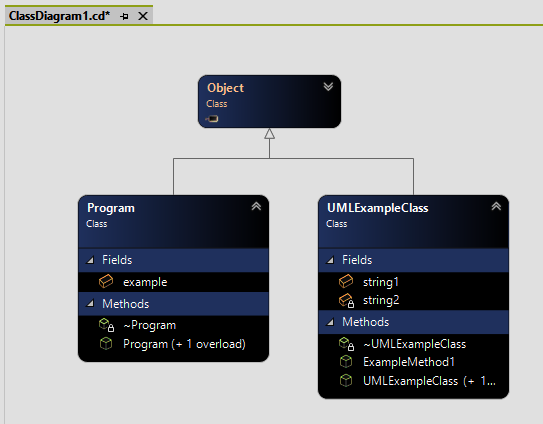
\includegraphics[width=6cm]{images/uml_vs.png}
	\caption{Ein von Visual Studio generiertes UML-Diagramm}
	\label{fig:uml_2}
\end{figure}
\FloatBarrier
Ein Werkzeug, welches unabhängig von der Programmierumgebung arbeitet, ist Doxygen. Es handelt sich um das Standard Werkzeug für die automatische Dokumentationsgenerierung. Einige der unterstützten Programmiersprachen sind C++, C, Objective-C, C\#, PHP, Java und Python \cite{Doxygen.2022}. 

Zur \textbf{Inline-Dokumentation} kann dagegen beispielhaft JavaDoc verwendet werden. Dieses ist in Intelij standardmäßig im Einsatz und verfügbar (siehe \autoref{code:codedescription}). 
\begin{lstlisting}[caption={Beispiel von Inline-Kommentaren}, label=code:codedescription]
	/**
	* Beschreibung der Methode
	* @param integer1 Beschreibung Parameter 1
	* @param integer2 Beschreibung Parameter 2
	* @return Beschreibung des zu retunierenden Wert
	*/
	public static String test(int integer1, int integer2){
		
		return "foo";
	}
\end{lstlisting}
\FloatBarrier
Die in \autoref{code:codedescription} verwendeten Kommentare erzeugen \autoref{fig:htmlBeschreibungMethode}. 
\begin{figure}
	\centering
	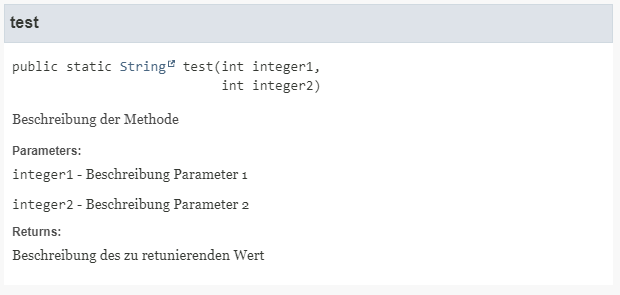
\includegraphics[width=10cm]{images/htmlBeschreibungMethode.png}
	\caption{Automatisch generierte Übersicht einer Java-Methode \autoref{code:codedescription}}
	\label{fig:htmlBeschreibungMethode}
\end{figure}
\FloatBarrier
Dennoch gibt es auch in diesem Feld weiter Anbieter, die eine Dokumentationserzeugung aus Inline-Kommentaren erlauben. Um den erwähnte XML-Standard aufzugreifen, ist hier Visual Studio zu erwähnen. In Visual Studio ist ein Bordmittel integriert, mit welchem sich die XML-Kommentare in eine HTML-Dokumentation wandeln lassen. Dazu gibt es verschiedene Schlüsselwörter, welche zur Beschreibung verwendet werden. So wird zum Beispiel das Schlüsselwort \textit{<summary>} zum Definieren einer Beschreibung eines bestimmten Elements verwendet werden. Des Weiteren können Parameter mit Kommentaren und Anmerkungen versehen werden. Dies geschieht mit dem Schlüsselwort \textit{<param name="nameDesParameters">Beschreibung des Parameters</param>}. 

Beim Verwenden der zwei Werkzeuge ist schon zu erkennen, dass sich das Prinzip nur leicht unterscheidet. Die Syntax und Semantik, mit welchen die Kommentare anzugeben sind, unterscheiden sich zwar im Format, jedoch ähneln sich die erzeugten Dokumentationen im Stil und Aufbau sehr. 

Doxygen, wie schon erwähnt (\autoref{subsubsec:diagramanalyses}), begrenzt sich nicht nur auf die UML-Diagrammerzeugung, sondern bietet auch in diesem Feld eine Lösung. Es kombiniert die Felder und gibt in der erzeugten Dokumentation sowohl die UML-Diagramme, als auch die einzeln definierten Beschreibungen an. Hierbei setzt Doxygen auf eigens definierte Befehle. Es gibt Befehle der Form \textit{\textbackslash Befehl} welche die Art des Kommentars beschreiben. Aber auch die erzeugte Dokumentation von Doxygen ähnelt den erwähnten Werkzeugen sehr. 

Eine Alternative, die für viele Programmiersprachen verwendet werden kann, ist Natural Docs. Natural Docs unterstützt 21 Programmiersprachen und ist folglich an keine Programmierumgebung gebunden. Dabei bindet sich Natural Docs wie Doxygen an keinen Stadard, sondern definiert seine eigenen Befehle zum Kommentieren.

Als ein bekanntes Beispiel einer automatisch generierten Dokumentation, bietet Oracle eine Dokumentation von Java\footnote{Vgl.: https://docs.oracle.com/javase/7/docs/api/overview-summary.html}. Dabei sind die einzelne Methoden, Klassen und Schnittstellen von den verschiedenen Java-Versionen dokumentiert.  
%% ggf. noch gituml falls ich noch was brauche - FW 15.11
%% + visual paradigme oder objectiFi

\subsection{Nutzen und Risiken}
Durch Werkzeuge zur Dokumentation werden Schritte des Prozesses automatisiert. Somit wird dieser weniger Fehleranfällig und einfacher anzuwenden. Durch die nun einfache Dokumentation sind Entwickler eher geneigt, ihren Code tatsächlich zu dokumentieren. Somit wird beispielsweise bei der Verwendung von dokumentierten Methoden klar, was die jeweilige Methode im Detail macht und worauf ggf. geachtet werden muss. Dies ist besonders bei großen Projekten wichtig, in welchen aufgrund getrennter Entwicklung regelmäßig fremde Methoden verwendet werden. So wird direkt bei den Vervollständigungsvorschlägen (siehe \autoref{sec:codecompletion}) die Inline-Dokumentation angezeigt. Außerdem müssen Diagramme nicht weiterhin von Hand erzeugt werden, sondern sind einfach exportierbar, sowie importierbar. 

Trotz aller Vorteile muss jedoch immer ein Mittelmaß gefunden werden. Gute Dokumentation ersetzt nicht \textit{Clean Code}, also beispielsweise die Verwendung von sinnvollen Namen. Außerdem muss darauf geachtet werden, dass Dokumentation auch bei Änderungen im Code aktuell gehalten wird. Ansonsten unterscheidet sich die Beschreibung von der tatsächlichen Funktionalität. Nicht zuletzt sollten Kommentare kurz und verständlich anstelle von lang und unübersichtlich sein. Ansonsten wird unnötig viel Zeit darauf verwendet und es fehlt eine einfache, schnelle Verständlichkeit. Eine übertriebene Nutzung der Kommentarfunktion kann den Quellcode sogar weniger leserlich machen. 

Bezüglich von Diagrammerzeugung muss außerdem erwähnt werden, dass gewisse Besonderheiten ggf. nicht automatisch in ein Diagramm übersetzt und somit manuell nachgebessert werden müssen. Erwähnenswert sind außerdem die möglicherweise anfallenden Kosten. Dies betrifft auch Werkzeuge zur Diagrammerzeugung aus Quelltexten wie in der Marktanalyse ersichtlich ist (\autoref{subsubsec:diagramanalyses}). 